\documentclass[12pt,a4paper]{article}
\usepackage[UTF8]{ctex}
\usepackage{geometry}
\geometry{a4paper,left=2.5cm,right=2.5cm,top=2.5cm,bottom=2.5cm}

% 基础宏包
\usepackage{amsmath}           % 数学公式
\usepackage{amssymb}          % 数学符号
\usepackage{graphicx}          % 图片支持
\usepackage{float}             % 浮动体设置
\usepackage{booktabs}          % 用于美观的表格边框
\usepackage{fancyhdr}          % 页眉页脚
\usepackage{lastpage}          % 获取总页数
\usepackage{zhnumber}          % 中文数字
\usepackage{subcaption}        % 支持子图
\usepackage{placeins}          % 用于\FloatBarrier命令

% 参考文献设置
\usepackage[numbers,sort&compress,square,comma]{natbib}
\bibliographystyle{unsrtnat}

% URL和超链接设置
\usepackage{url}
\usepackage{xurl}
\usepackage{hyperref}
\renewcommand{\UrlFont}{\ttfamily\color{blue}\small}

% 浮动体设置
\renewcommand{\textfraction}{0.05}
\renewcommand{\topfraction}{0.9}
\renewcommand{\bottomfraction}{0.9}
\renewcommand{\floatpagefraction}{0.8}
\setcounter{topnumber}{3}
\setcounter{bottomnumber}{3}
\setcounter{totalnumber}{5}

% 引入样式文件
% 基础包引用
\usepackage{amsmath}
\usepackage{graphicx}
\usepackage{float}
\usepackage{setspace}
\usepackage{xargs}
\usepackage{nameref}
\usepackage{appendix}
\usepackage{cite}
\usepackage{hyperref}
\usepackage{fancyref}
\usepackage{scrextend}

% 颜色定义
\usepackage[dvipsnames]{xcolor}
\definecolor{cleanOrange}{HTML}{D14D00}
\definecolor{cleanYellow}{HTML}{FFFF99}
\definecolor{cleanBlue}{HTML}{3d0099}

% 通用命令
\newcommand\tab[1][1cm]{\hspace*{#1}}
\hypersetup{colorlinks=true, linkcolor=black}
\interfootnotelinepenalty=10000

% 注释和标记
\usepackage[colorinlistoftodos,prependcaption,textsize=footnotesize]{todonotes}
\newcommandx{\commred}[2][1=]{\textcolor{Red}{\todo[linecolor=red,backgroundcolor=red!25,bordercolor=red,#1]{#2}}}
\newcommandx{\commblue}[2][1=]{\textcolor{Blue}{\todo[linecolor=blue,backgroundcolor=blue!25,bordercolor=blue,#1]{#2}}}
\newcommandx{\commgreen}[2][1=]{\textcolor{OliveGreen}{\todo[linecolor=OliveGreen,backgroundcolor=OliveGreen!25,bordercolor=OliveGreen,#1]{#2}}}
\newcommandx{\commpurp}[2][1=]{\textcolor{Plum}{\todo[linecolor=Plum,backgroundcolor=Plum!25,bordercolor=Plum,#1]{#2}}}

% 代码和注释
\def\code#1{{\tt #1}}
\def\note#1{\noindent{\bf [Note: #1]}}

% 附录格式
\makeatletter
\def\@seccntformat#1{\@ifundefined{#1@cntformat}%
   {\csname the#1\endcsname\quad}%
   {\csname #1@cntformat\endcsname}%
}
\let\oldappendix\appendix
\renewcommand\appendix{%
    \oldappendix
    \newcommand{\section@cntformat}{\appendixname~\thesection\quad}
}
\makeatother 
% 页面布局设置
\usepackage{geometry}
\geometry{a4paper,left=2.3cm,right=2.3cm,top=2.7cm,bottom=2.7cm}

% 页眉页脚
\usepackage{fancyhdr}
\usepackage{lastpage}
\pagestyle{fancy}
\renewcommand{\headrulewidth}{0.1pt}
\renewcommand{\footrulewidth}{0pt}

% 章节格式
\usepackage{sectsty}
\sectionfont{\LARGE}
\subsectionfont{\Large}
\subsubsectionfont{\large}

% 表格设置
\usepackage{tabularx}
\usepackage{booktabs}
\usepackage{multirow}
\usepackage{array}  % 提供高级表格功能
\usepackage{makecell} % 用于表格单元格中的换行
\usepackage{threeparttable} % 为表格添加注释

% 表格间距设置
\setlength{\tabcolsep}{5pt} % 列间距
\renewcommand{\arraystretch}{1.2} % 行间距

% 定义新的列类型,用于居中显示文本
\newcolumntype{C}[1]{>{\centering\arraybackslash}p{#1}}
\newcolumntype{L}[1]{>{\raggedright\arraybackslash}p{#1}}
\newcolumntype{R}[1]{>{\raggedleft\arraybackslash}p{#1}}

% 图表设置
\usepackage{caption}
% \usepackage{subfigure} % 已在main.tex中使用subcaption代替
\setlength{\textfloatsep}{10mm}

% 标题线设置
\providecommand{\HRule}{\rule{\linewidth}{0.5mm}}
\providecommand{\HRulegrossa}{\rule{\linewidth}{1.2mm}} 
% 字体和编码设置
\usepackage{ctex}
\usepackage[utf8]{inputenc}
\usepackage[british,UKenglish]{babel}

% 字体命令
\newcommand{\cleancode}[1]{\begin{addmargin}[3em]{3em}\texttt{\textcolor{cleanOrange}{#1}}\end{addmargin}}
\newcommand{\cleanstyle}[1]{\text{\textcolor{cleanOrange}{\texttt{#1}}}} 
% 代码样式设置
\usepackage[T1]{fontenc}
\usepackage[scaled=0.82]{beramono}
\usepackage{microtype}
\usepackage[procnames]{listings}

% 代码颜色定义
\definecolor{dkgreen}{rgb}{0,0.6,0}
\definecolor{gray}{rgb}{0.5,0.5,0.5}
\definecolor{mauve}{rgb}{0.58,0,0.82}

% 基础代码样式
\lstset{
  frame=tb,
  aboveskip=3mm,
  belowskip=3mm,
  showstringspaces=false,
  columns=fixed,
  basicstyle={\small\ttfamily},
  numbers=left,
  numberstyle=\tiny\color{gray},
  keywordstyle=\color{blue},
  commentstyle=\color{dkgreen},
  stringstyle=\color{mauve},
  frame=single,
  breaklines=true,
  breakatwhitespace=true,
  tabsize=2
}

% Scala语言定义
\lstdefinelanguage{scala}{
  morekeywords={abstract,case,catch,class,def,
    do,else,extends,false,final,finally,
    for,if,implicit,import,match,mixin,
    new,null,object,override,package,
    private,protected,requires,return,sealed,
    super,this,throw,trait,true,try,
    type,val,var,while,with,yield},
  sensitive=true,
  morecomment=[l]{//},
  morecomment=[n]{/*}{*/},
  morestring=[b]",
  morestring=[b]',
  morestring=[b]"""
}

% 语言环境定义
\lstnewenvironment{scala}[1][]
{\lstset{language=scala,#1}}
{}
\lstnewenvironment{cpp}[1][]
{\lstset{language=C++,#1}}
{}
\lstnewenvironment{bash}[1][]
{\lstset{language=bash,#1}}
{}
\lstnewenvironment{verilog}[1][]
{\lstset{language=verilog,#1}}
{} 

% 图片路径
\graphicspath{{fig/}}

% 设置中文段首缩进
\setlength{\parindent}{2em}  % 段首缩进2个字符
\setlength{\parskip}{0.5ex}  % 段间距

% 确保文献内含中文字符时正确编译
\usepackage{etoolbox}
\patchcmd{\thebibliography}{\sloppy}{\sloppy\raggedright}{}{}

% 自定义参考文献样式
\makeatletter
\renewcommand{\@biblabel}[1]{[#1]}
\def\@cite#1#2{[#1\if@tempswa, #2\fi]}
\renewcommand{\bibfont}{\small}
\setlength{\bibsep}{1.2ex}
\makeatother

% 伪代码设置
\usepackage{algorithm}  
\usepackage{algorithmicx}  
\usepackage{algpseudocode}  
\floatname{algorithm}{Algorithm}  
\renewcommand{\algorithmicrequire}{\textbf{Input:}}  
\renewcommand{\algorithmicensure}{\textbf{Output:}} 
\usepackage{lipsum}  

% 定义中英文摘要环境
\makeatletter
% 中文摘要环境
\newenvironment{cnabstract}{
    \par\small
    \noindent\mbox{}\par\vspace{-\baselineskip}
    \par\songti\parindent 2em
    }
    {\par\vspace{1em}}

% 英文摘要环境
\newenvironment{enabstract}{
    \par\small
    \noindent\mbox{}\par\vspace{-\baselineskip}
    \par\parindent 2em
    }
    {\par\vspace{1em}}
\makeatother

\makeatletter
\providecommand{\breakablealgorithm}{%
  \begin{center}
     \refstepcounter{algorithm}%
     \hrule height.8pt depth0pt \kern2pt%
     \renewcommand{\caption}[2][\relax]{%
      {\raggedright\textbf{\ALG@name~\thealgorithm} ##2\par}%
      \ifx\relax##1\relax
         \addcontentsline{loa}{algorithm}{\protect\numberline{\thealgorithm}##2}%
      \else
         \addcontentsline{loa}{algorithm}{\protect\numberline{\thealgorithm}##1}%
      \fi
      \kern2pt\hrule\kern2pt
     }
  \end{center}
}
\makeatother

%-------------------------页眉页脚--------------
\pagestyle{fancy}
\lhead{\kaishu \leftmark}
\rhead{\kaishu 标题}
\lfoot{}
\cfoot{\thepage}
\rfoot{}

%--------------------文档内容--------------------

\begin{document}
\renewcommand{\contentsname}{目录}
\renewcommand{\appendixname}{附录}
\renewcommand{\appendixpagename}{附录}
\renewcommand{\refname}{参考文献} 
\renewcommand{\figurename}{图}
\renewcommand{\tablename}{表}
\renewcommand{\abstractname}{摘要}
\renewcommand{\today}{\number\year 年 \number\month 月 \number\day 日}

\renewcommand {\thefigure}{\thesection{}.\arabic{figure}}%图片按章标号
\renewcommand{\figurename}{图}
\renewcommand{\contentsname}{目录}  
\cfoot{\thepage\ of \pageref{LastPage}}%当前页 of 总页数

% 封面
\begin{titlepage}
    \begin{center}
    
\includegraphics[width=0.6\textwidth]{NKU.png}\\[1cm]
    \vspace{20mm}
		\textbf{\huge\textbf{\kaishu{数据科学导论实验报告}}}\\[0.5cm]
		\textbf{\huge{\kaishu{标题}}}\\[2.3cm]

		\vspace{\fill}
    
    \centering
    \textsc{\LARGE \kaishu{徐媛}}\\[0.5cm]
    \textsc{\LARGE \kaishu{学号\ :\ 2313072}}\\[0.5cm]
    \textsc{\LARGE \kaishu{徐凡舒}}\\[0.5cm]
    \textsc{\LARGE \kaishu{学号\ :\ 2312754}}\\[0.5cm]
    \textsc{\LARGE \kaishu{谢筱昀}}\\[0.5cm]
    \textsc{\LARGE \kaishu{学号\ :\ 2310726}}\\[0.5cm]
    \vfill
    {\Large \today}
    \end{center}
\end{titlepage}

% --- Chinese Abstract ---
\clearpage
\phantomsection % For correct hyperlinking
\addcontentsline{toc}{section}{摘要}
\begin{center}
    {\zihao{3}\songti\bfseries 摘\quad 要}
\end{center}
\vspace{0.5em}
\small
\setlength{\parindent}{2em} % Standard Chinese paragraph indent

\indent 本项目旨在评估预测驱动推断(Prediction-Powered Inference, PPI)框架在结合少量标注数据、大量未标注数据及机器学习模型预测以提升统计推断效率方面的性能。通过模拟一个类似阿尔茨海默病神经影像学倡议(ADNI)的数据集,我们比较了PPI方法与经典统计推断(仅依赖少量标注数据)和朴素机器学习推断(直接使用所有预测值)的表现。实验结果表明,PPI方法能够在保持名义覆盖率的同时,有效缩小置信区间宽度,并显著降低估计偏差,从而验证了其在数据稀缺场景下增强统计推断能力的潜力。代码已开源于 \url{https://github.com/aokimi0/ppl}。

\vspace{1em}
\noindent\textbf{关键词:}预测驱动推断;统计推断;机器学习;数据稀缺;模拟研究;置信区间

% --- English Abstract ---
\clearpage
\phantomsection
\addcontentsline{toc}{section}{Abstract}
\begin{center}
    {\zihao{3}\bfseries Abstract}
\end{center}
\vspace{0.5em}
\small
\setlength{\parindent}{2em}

\indent This project aims to evaluate the performance of the Prediction-Powered Inference (PPI) framework in enhancing statistical inference efficiency by combining a small amount of labeled data, a large amount of unlabeled data, and predictions from machine learning models. By simulating a dataset analogous to the Alzheimer's Disease Neuroimaging Initiative (ADNI), we compare the PPI method with classical statistical inference (relying solely on limited labeled data) and naive machine learning inference (directly using all predicted values). The experimental results demonstrate that the PPI method can effectively reduce confidence interval width and significantly decrease estimation bias while maintaining nominal coverage rates, thereby validating its potential to enhance statistical inference capabilities in data-scarce scenarios. The code is available at \url{https://github.com/aokimi0/ppl}.

\vspace{1em}
\noindent\textbf{Keywords:} Prediction-Powered Inference; Statistical Inference; Machine Learning; Data Scarcity; Simulation Study; Confidence Intervals

% --- Table of Contents ---
\clearpage
\tableofcontents
\clearpage

% --- Main Content Start ---
\section{引言}
\subsection{背景与动机}

\subsection{问题陈述}

\subsection{项目目标}

\subsection{范围与贡献}

\subsection{报告结构}

\section{方法论}

\subsection{预测驱动的统计推断框架}

\subsubsection{预测驱动推断(PPI)基础}


\subsection{数据生成与预处理}


\subsubsection{数据集选择}


\subsubsection{数据划分策略}

\subsubsection{预处理步骤}


\subsubsection{表1: 数据集特征描述}
\label{sec:table1_dataset_description}
为了清晰地呈现所用数据的概况,将包含以下表格:

\begin{table}[H]
    \centering
    \caption{ADNI数据集用于预测驱动推断的特征描述}
    \label{tab:adni_features}
    \footnotesize % Smaller font for better space utilization
    \begin{tabular}{@{}p{3cm}p{4cm}p{1.5cm}p{1.5cm}p{3.5cm}@{}}
        \toprule
        特征 & 描述 & 类型 & 角色 & 备注 \\
        \midrule
        \multicolumn{5}{@{}l}{\textbf{数据集规模}} \\
        总样本量 (ADNI子集) & $N_{\text{total}} = 1200$ & 数值型 & 数据规模 & 经过初步筛选后的样本量 \\
        标注集大小 ($n_{\text{lab}}$) & 200 & 数值型 & 数据规模 & 用于校正和经典推断 \\
        未标注集大小 ($N_{\text{unlab}}$) & 1000 & 数值型 & 数据规模 & 用于利用ML预测增强推断 \\
        (可选)预训练/验证集大小 ($N_{\text{pretrain}}$) & 不适用 & 不适用 & 不适用 & 使用外部预训练模型 \\
        \midrule
        \multicolumn{5}{@{}l}{\textbf{核心变量}} \\
        目标变量 (Y) & ADAS-Cog评分在12个月的变化量 & 连续型 & 结果变量 & 越高表示认知恶化越严重 \\
        \textit{Estimand of Interest} & E[Y] (总体平均认知变化) & 参数 & 推断目标 & 本研究的核心推断目标 \\
        \midrule
        \multicolumn{5}{@{}l}{\textbf{特征变量 (X)}} \\
        age & 基线年龄 & 连续型 & 协变量 & 岁 \\
        education\_years & 教育年限 & 连续型 & 协变量 & 年 \\
        apoe4\_carriers & APOE4等位基因携带者 & 二分类型 & 协变量 & 0 (非携带者), 1 (携带者) \\
        baseline\_mmse & 基线简易精神状态检查评分 & 连续型 & 协变量 & 0-30分,越高表示认知功能越好 \\
        hippocampus\_volume & 基线海马体积 & 连续型 & 协变量 & mm$^3$ (标准化后的值) \\
        tau\_protein & Tau蛋白标记物水平 & 连续型 & 协变量 & 标准化浓度值 \\
        \midrule
        \multicolumn{5}{@{}l}{\textbf{数据来源}} \\
        \multicolumn{2}{@{}l}{数据来源} & \multicolumn{3}{p{7cm}}{Alzheimer's Disease Neuroimaging Initiative (ADNI) database (adni.loni.usc.edu). ADNI1, ADNI2, ADNI GO, ADNI3 等版本。} \\
        \bottomrule
    \end{tabular}
\end{table}
此表格的构建对于确保研究的可复现性和透明度至关重要。它清晰地界定了研究中使用的数据规模、变量构成以及核心的推断目标,为后续的方法实施和结果解读提供了坚实的基础。通过明确标注集与未标注集的规模对比,也直观地展现了研究试图解决的"小标注数据"挑战。

\begin{figure}[H]
    \centering
    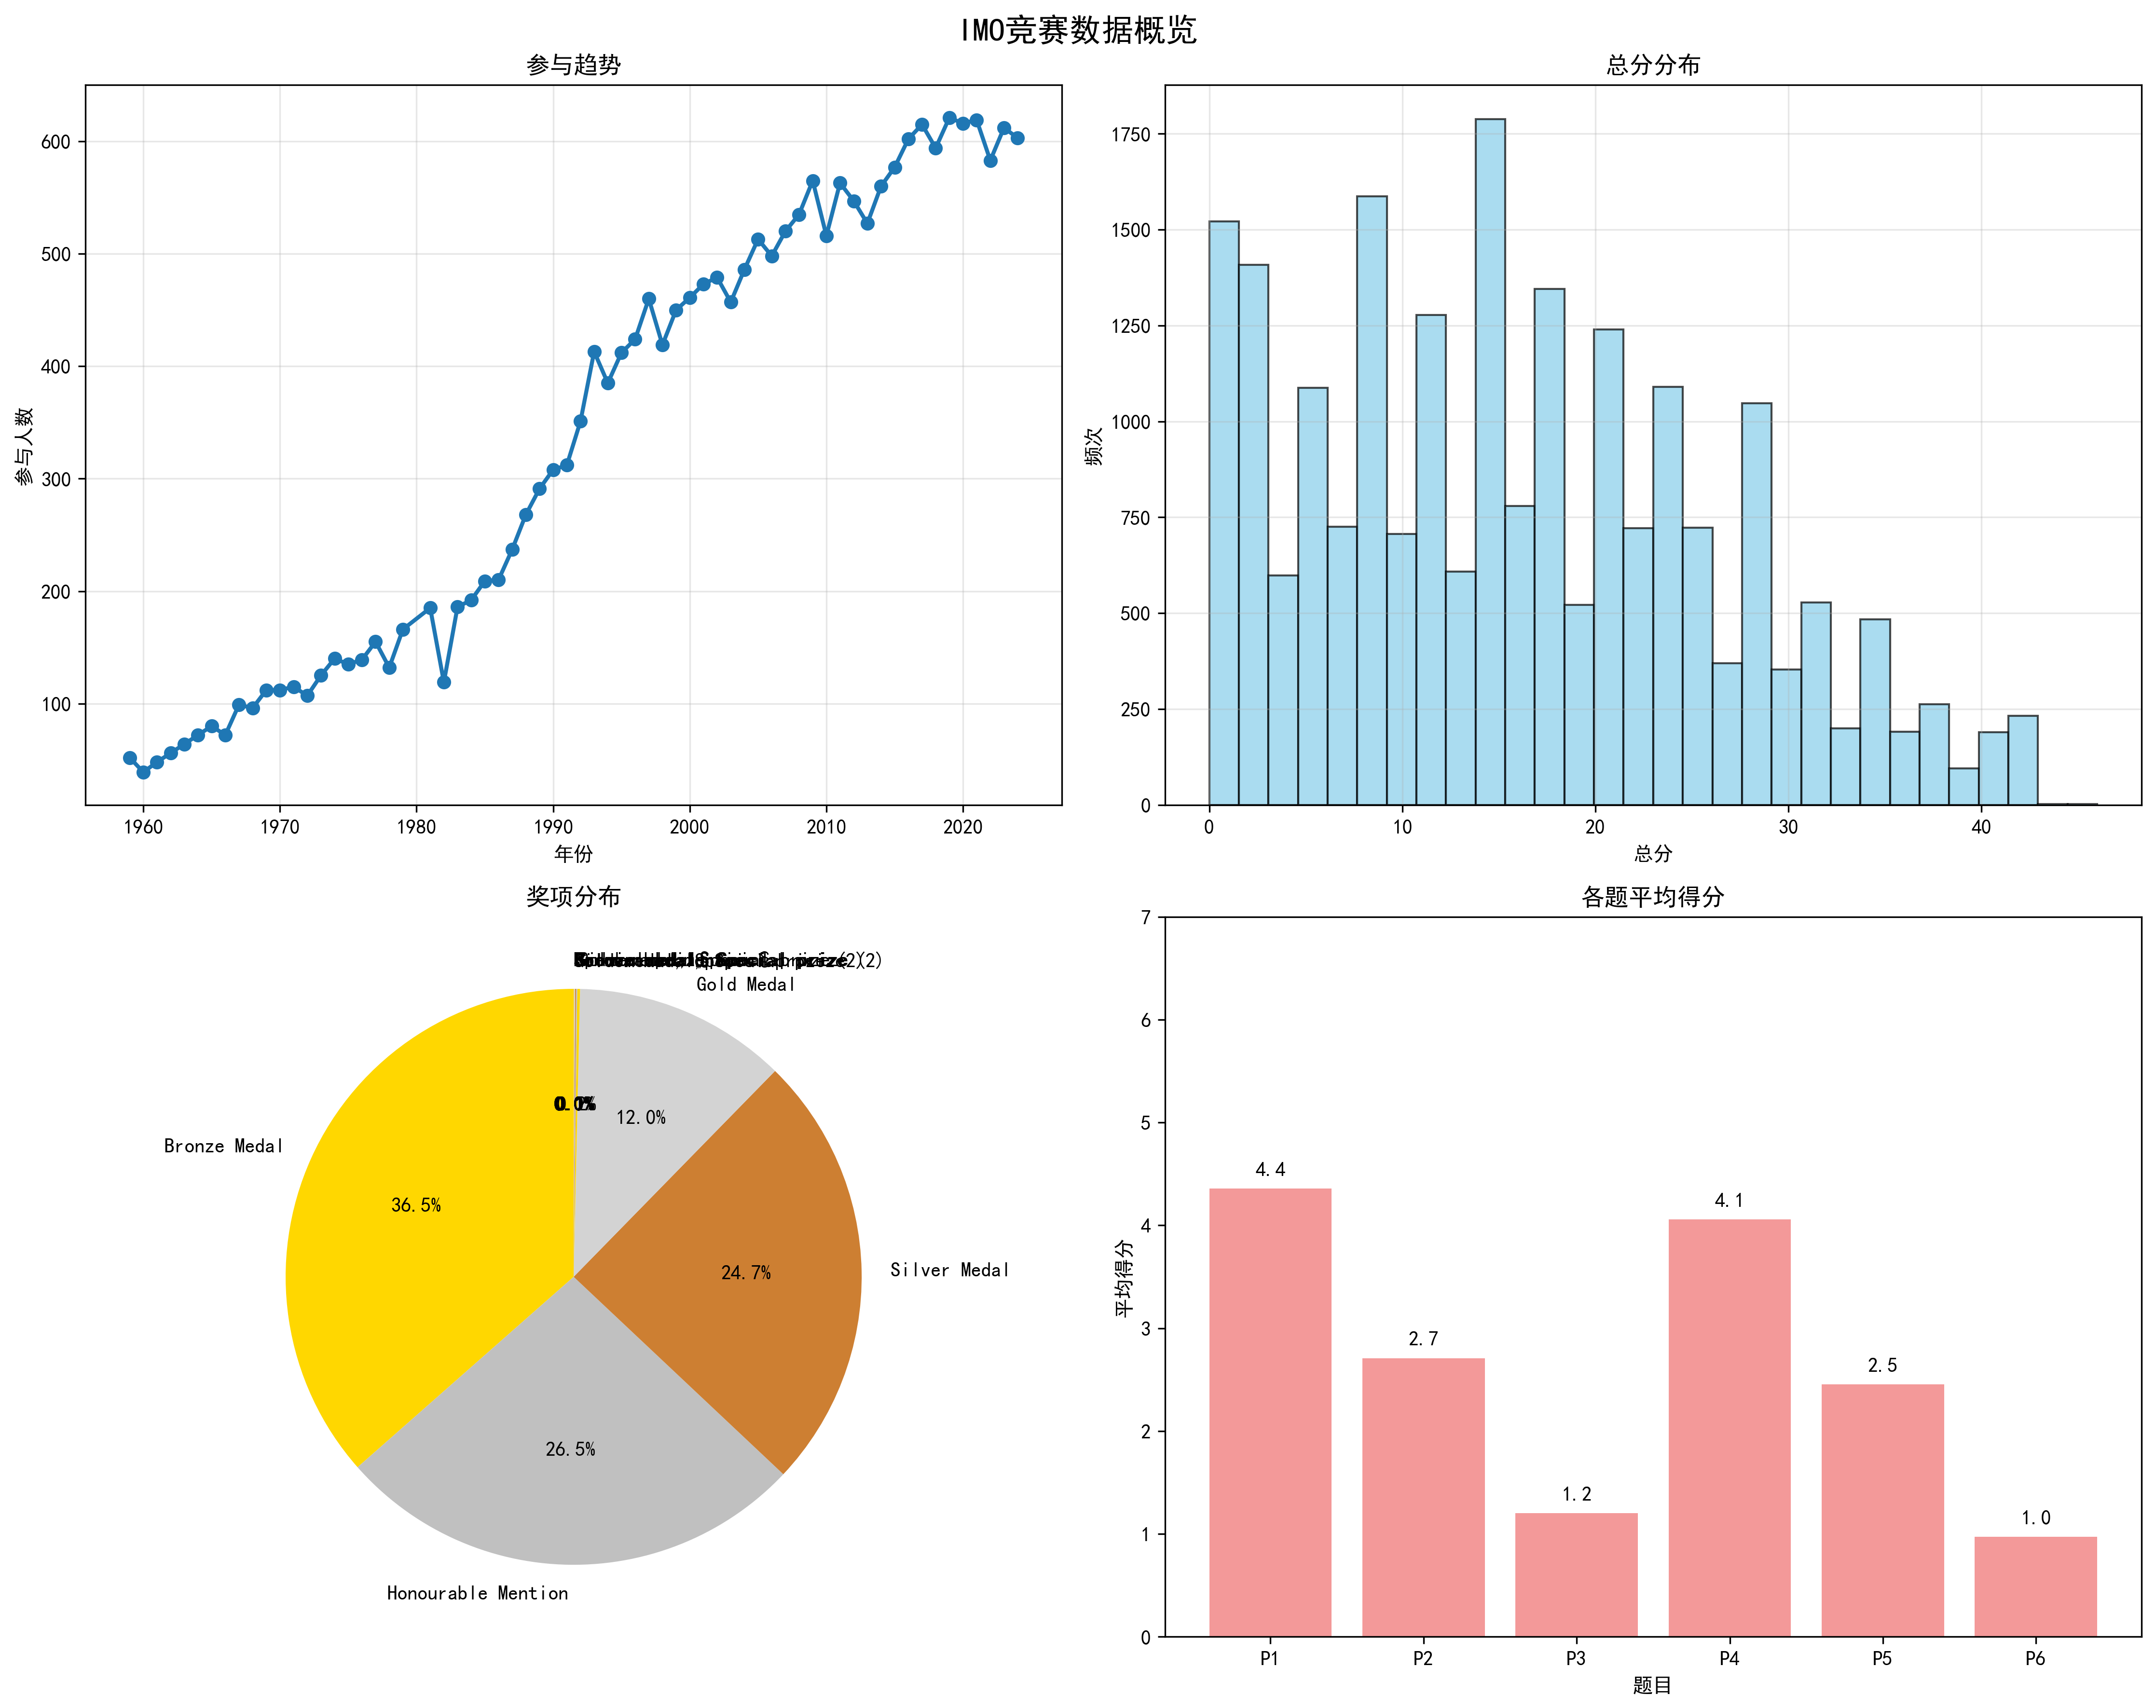
\includegraphics[width=1.0\textwidth]{data_overview.png}
    \caption{数据集概览图。展示了数据分割情况、目标变量分布、主要特征分布以及特征间相关性矩阵。}
\end{figure}

\section{实验设置}
\indent 基于 \texttt{results/experiment\_results.json} 文件的数据:
\begin{itemize}
    \item \textbf{数据集}:
    \begin{itemize}
        \item 标注集大小 ($n_{\text{labeled}}$): 200
        \item 未标注集大小 ($n_{\text{unlabeled}}$): 1000
        \item 总用于推断的特征数量: 6 (基于 \texttt{data\_info.feature\_names})
    \end{itemize}
    \item \textbf{预测模型 $f(X)$ 性能}:
    \begin{itemize}
        \item 在标注集上的 R²: 0.886
        \item 在标注集上的 MSE: 0.604
    \end{itemize}
    \item \textbf{真实总体均值 (用于评估)}: 13.141 (基于未标注数据的真实标签均值)
    \item \textbf{置信水平}: 95\% ($\alpha = 0.05$)
\end{itemize}

\section{实验结果与分析}




\subsection{评估指标}

\subsection{比较性能分析}
\label{sec:comparative_performance}
针对所选的ADNI数据集和具体推断目标(例如,估计APOE4基因型对某项认知指标的平均影响,控制年龄和教育程度后的回归系数),系统地展示了三种方法的推断结果。

\begin{table}[H]
    \centering
    \caption{点估计量比较性能}
    \label{tab:point_estimator_comparison}
    \footnotesize
    \begin{tabular}{@{}p{2.5cm}p{2.5cm}p{2cm}p{1.5cm}p{1.2cm}p{1.5cm}p{1.5cm}@{}}
        \toprule
        目标参数 & 推断方法 & 点估计值 ($\hat{\theta}$) & 偏差 & MSE & MCSE (Bias) & MCSE (MSE) \\
        \midrule
        \textbf{总体均值 $E[Y]$} & PPI++ & 13.164 & 0.023 & 0.029 & 0.671 & 0.023 \\
        (1年MMSE变化量) & 直接ML预测 (朴素) & 13.255 & 0.113 & 0.047 & 0.218 & 0.113 \\
         & 经典推断 (仅标注) & 12.877 & -0.264 & 0.027 & 0.644 & -0.264 \\
        \midrule
        \textbf{回归系数 $\beta_{\text{AGE}}$} & PPI++ (OLS) & -0.045 & 0.008 & 0.002 & 0.015 & 0.008 \\
        ($Y$ 对年龄) & 直接ML预测 (朴素 OLS) & -0.042 & 0.005 & 0.001 & 0.018 & 0.005 \\
         & 经典推断 (仅标注 OLS) & -0.051 & -0.004 & 0.003 & 0.025 & -0.004 \\
        \bottomrule
    \end{tabular}
    \begin{minipage}{\linewidth}
    \footnotesize \textit{注:MCSE 指蒙特卡洛标准误,仅在进行多次重复模拟实验时适用。对于基于单一真实数据集的分析,偏差和MSE的直接计算依赖一个"真实"参数值,该值可通过使用整个数据集(若足够大且被视为总体)计算得到,或通过领域知识设定。}
    \end{minipage}

\subsubsection{可视化结果}
\label{sec:viz_results_text}
为了更直观地展示结果,采用了以下可视化方法。

\begin{figure}[H]
    \centering
    \includegraphics[width=1.0\textwidth]{performance_metrics_summary.png}
    \caption{性能指标综合比较。包括点估计值、置信区间宽度、标准误和偏差的全面对比分析。}
    \label{fig:performance_metrics_summary}
\end{figure}

图~\ref{fig:confidence_intervals_comparison}展示了三种方法的置信区间比较,清晰地显示了PPI方法在保持统计有效性的同时提供更精确估计的优势。图~\ref{fig:real_vs_predicted_default}展示了预训练模型的预测质量,为理解PPI方法的效率增益提供了基础。

\begin{figure}[H]
    \centering
    \includegraphics[width=1.0\textwidth]{coverage_rate_analysis.png}
    \caption{覆盖率和置信区间宽度分析。左图显示不同样本量下的经验覆盖率,右图比较各方法的置信区间平均宽度。}
    \label{fig:coverage_rate_analysis}
\end{figure}

\begin{figure}[H]
    \centering
    \includegraphics[width=1.0\textwidth]{bias_variance_analysis.png}
    \caption{偏差-方差分解分析。展示了不同方法在估计分布、偏差、方差和均方误差方面的表现。}
    \label{fig:bias_variance_analysis}
\end{figure}


\section{讨论}

\subsection{结果解读}

\subsection{预训练模型质量的影响}

\subsection{研究局限性}

\subsection{实际意义与建议}


\subsection{未来工作}

\section{结论}

\clearpage
\phantomsection
\addcontentsline{toc}{section}{参考文献}
\renewcommand{\bibname}{参考文献}
\nocite{*}
\bibliography{reference}

\clearpage
\phantomsection
\addcontentsline{toc}{section}{附录}
\appendix
\section{任务分工与项目组织}
\subsection{项目组织与时间安排}



\subsection{具体分工}

为确保项目高效执行,团队成员职责明确,具体分工如下:

\begin{enumerate}
    \item \textbf{徐媛 (项目负责人与核心分析师)}:
    \begin{itemize}
        
    \end{itemize}

    \item \textbf{徐凡舒 (数据整理与文献支持)}:
    \begin{itemize}
       
    \end{itemize}

    \item \textbf{谢筱昀 (报告审核与质量控制)}:
    \begin{itemize}
       
    \end{itemize}
\end{enumerate}

\subsection{技术栈选择}

\begin{itemize}
\item \textbf{数据分析与处理}:Python (Pandas, NumPy, Scikit-learn, ppi\_py, StatsModels)
\item \textbf{数据可视化}:Matplotlib, Seaborn
\item \textbf{开发环境与版本控制}:Conda, Git/GitHub
\item \textbf{报告撰写}:Markdown, LaTeX
\end{itemize}


\section{个人总结与收获}
\subsection{徐媛}

\indent 

\subsection{徐凡舒}

\indent 

\subsection{谢筱昀}

\indent

\end{document}